\section{专用加速器：systolic array、TPU 与 Trainium}
\label{sec:accel}

既然 GPU 已经很快，为什么 Google、AWS 还要自己做芯片？答案在能耗上。通用处理器把大部分能耗花在取指、译码、调度和数据搬运上，
真正做运算的部分只占一小份。Horowitz 在 45~nm 工艺下的测量表明，一次 DRAM 访问的能耗比一次 32 位浮点乘法高两个数量级以上，
而 8 位整数乘法又比 FP32 乘法便宜一个数量级以上~\cite{horowitz2014energy}。所以专用加速器只有两条路可走~\cite{dally2020domain,sze2017efficient}：
一是把控制开销摊到大量运算上（宽 SIMD、矩阵单元），二是把数据留在离运算最近的地方反复使用。
这两条路可以用同一个量来衡量：每从 DRAM 取一个字，能做多少次运算。这正是 roofline 里的算术强度。

\subsection{Systolic array 与数据流}

Kung 提出的 systolic 架构~\cite{kung1982systolic} 让数据像心跳一样，在规则排列的处理单元（PE）之间一拍一拍地流动，每个 PE 只和邻居通信。
用 $P\times P$ 的阵列算矩阵乘时，$A$ 的一个元素从左侧进入，向右流过 $P$ 个 PE，被复用了 $P$ 次。只有阵列的边界需要读存储，
所以片上带宽需求从 $O(P^2)$ 降到了 $O(P)$。按照哪个操作数常驻在 PE 里，可以分出三种数据流~\cite{chen2016eyeriss,sze2017efficient}：
weight-stationary 让权重常驻，激活横向流动、部分和纵向流动，代表是 TPU v1；output-stationary 让每个 PE 固定累加一个输出；
row-stationary 是 Eyeriss 的做法，把卷积的一行权重和对应的输入一起留在 PE 中。

阵列的代价是填充和排空。对 weight-stationary 阵列来说，一个 $P\times P$ 的权重块处理 $M$ 行输入需要 $M+2P-2$ 个周期；
如果权重加载不和计算重叠，还要再加 $P$ 个周期，利用率约为 $M/(M+3P-2)$。也就是说，矩阵必须比阵列大得多，开销才摊得薄。
\lab{CS149 A4}用寄存器级仿真按周期精确地验证了这个公式（图~\ref{fig:labkvsys} 中）。$P=16$ 时，$n=16$ 的矩阵利用率只有 0.258；
$n=64$ 时，串行加载权重为 0.582，权重做双缓冲后升到 0.957。反过来固定 $n=128$，$P=4$ 的阵列利用率是 0.928，$P=128$ 只有 0.251：
矩阵只有一个块时，双缓冲也救不回来。

\begin{figure*}[!t]
\centering
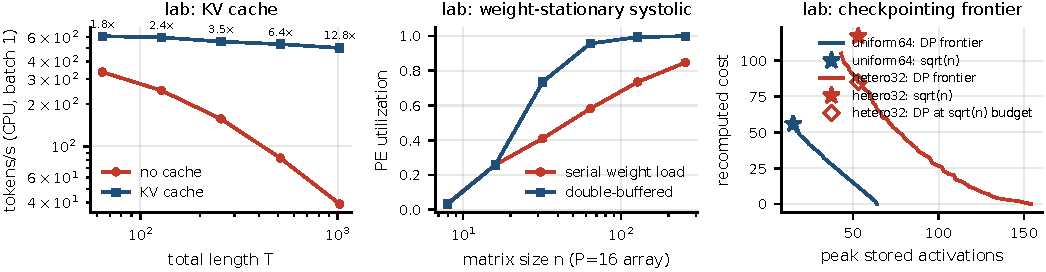
\includegraphics[width=\textwidth]{fig_lab_kv_systolic}
\caption{本文配套实验（CPU 测量与寄存器级仿真）。左：本地训练的 0.8M 参数 nanoGPT（4 层、宽 128）在 CPU、batch 1 下有无 KV cache 的生成吞吐。加速比从 $T=64$ 的 1.8 倍增长到 $T=1024$ 的 12.8 倍，
因为没有 cache 时每一步都要重算整个前缀，总代价是 $O(T^2)$。中：$16\times16$ weight-stationary systolic 阵列的 PE 利用率随矩阵尺寸的变化；权重双缓冲在 $n\ge64$ 时把利用率推到 0.95 以上，因为加载权重的周期被藏到了计算后面。
右：激活重计算的「峰值存储--重算代价」前沿，星号是 $\sqrt{n}$ 均匀分段，菱形是同一预算下动态规划的解。}
\label{fig:labkvsys}
\end{figure*}

\begin{qa}{Systolic array 为什么适合矩阵乘？缺点是什么？}
\ans 因为矩阵乘里每个操作数都要参与 $O(n)$ 次运算，systolic 阵列让这种复用发生在相邻 PE 的寄存器之间：从 SRAM 读一次的数被用 $P$ 次，
控制逻辑又极少，所以能效很高。缺点有两个。矩阵比阵列小或形状不匹配时，$3P-2$ 的填充排空开销摊不薄，利用率低；
对 softmax、归约、gather 这类非 GEMM 运算也不友好，需要额外的向量和标量单元。
\wrong 「TPU 快是因为频率高」。TPU v1 的频率只有 700~MHz。
\end{qa}

\begin{qa}{weight-stationary 和 output-stationary 怎么选？}
\ans 看哪个操作数复用最多、哪个最大。推理时同一份权重要乘 batch 里的每个样本，让权重常驻就能把权重读取摊到整个 batch 上，适合 batch（$M$）大的场景。
output-stationary 让部分和一直留在 PE 里，省掉部分和的往返，适合收缩维 $K$ 很长、输出较小的场景。
\wrong 「两者只是实现细节，性能一样」。
\end{qa}

\subsection{TPU：从推理 ASIC 到光互联超级计算机}

TPU v1~\cite{jouppi2017tpu} 是一颗推理芯片：$256\times256=65536$ 个 8 位 MAC，频率 700~MHz，峰值约 92~TOPS；
片上有 28~MiB 软件管理的存储（24~MiB unified buffer 加 4~MiB 累加器），权重来自 8~GiB 的 DDR3，带宽 34~GB/s。
这篇论文最有价值的部分不是峰值，而是它的 roofline 分析。线上负载以 MLP 和 LSTM 为主，它们的权重复用程度取决于 batch；
而 P99 时延约束（MLP0 为 7~ms）限制了 batch 不能太大。结果大多数应用都落在 roofline 的斜线段上，受权重带宽限制，只有 CNN 接近计算屋顶。

\begin{est}{TPU v1 的拐点与所需 batch}
峰值是 $65536\times2\times700\,\text{MHz}\approx92$~TOPS，权重带宽 34~GB/s，拐点就是 $92\times10^{12}/34\times10^{9}\approx2700$~ops/B。
INT8 的 MLP 在 batch 为 $B$ 时，每个权重字节做 $2B$ 次运算，所以要 $B\ge1350$ 才受算力限制。线上的 batch 远小于这个数。
这和今天 LLM decode 受 HBM 带宽限制是同一个现象，只是拐点从 2700 换成了 H100 的 295。
\end{est}

之后的 TPU 走向了大规模训练。TPU v4~\cite{jouppi2023tpuv4} 用光路交换机（OCS）把 4096 颗芯片连成可重构的 3D torus，并加入了面向 embedding 的 SparseCore；
每颗芯片的 BF16 峰值是 275~TFLOP/s，配 32~GiB HBM2，带宽约 1.2~TB/s。它的主要编程接口是 XLA 和 GSPMD~\cite{xu2021gspmd}：
程序员给张量加上 sharding 注解，由编译器插入集合通信。

\subsection{AWS Trainium 与 NKI}

Trainium 代表了另一种思路：把片上存储完全交给软件管理。Trainium（Trn1）的 NeuronCore-v2 包含 Tensor Engine（$128\times128$ 的 systolic array）、
Vector Engine、Scalar Engine 和 GpSimd Engine。片上存储分两级：SBUF（24~MiB，分 128 个 partition）存放输入和输出 tile，
PSUM（2~MiB）是矩阵乘的累加缓冲~\cite{awsneuron}。NKI（Neuron Kernel Interface）是一种嵌在 Python 里的 kernel 语言。
在 NKI 中，tile 的第 0 维是 partition 维，最大 128，对应阵列的一条边；\texttt{nc\_matmul} 沿 partition 维做收缩，结果写入 PSUM；
HBM 和 SBUF 之间的搬运全部是显式 DMA。CS149 Fall 2024 的作业 4 就是在这套硬件上手工分块卷积和矩阵乘，体会 tile 形状对利用率的影响。
和 GPU 的 shared memory 不同，这里没有 L1/L2 兜底，所有复用都必须显式写出来，写错了就直接撞上 DRAM 带宽墙。

显式化是有代价的。\lab{CS149 A4}测量了 im2col：它把卷积展开成 GEMM，数据膨胀倍数约为 $K_HK_W/\text{stride}^2$，
ResNet conv1（$7\times7$、stride 2）是 12.25 倍。在 numpy 中，im2col 加 GEMM 仍比逐 tap 的直接卷积快，但 $3\times3$ 层有 73\% 的时间花在拷贝 patch 矩阵上；
$1\times1$ 卷积没有膨胀，直接卷积反而更快。GPU 上的 implicit GEMM 和 Winograd 就是为了避开这种显式膨胀。

\begin{table*}[!t]
\centering
\caption{代表性 ML 加速器对比（数字取自论文与官方文档；拐点 = 峰值 / 片外带宽）}
\label{tab:accel}
\footnotesize
\begin{tabularx}{\textwidth}{@{}l L{2.6cm} L{2.8cm} L{3.0cm} Y Y@{}}
\toprule
加速器 & 计算单元 & 片上存储 & 片外存储与峰值 & 编程模型 & 面试要点 \\
\midrule
NVIDIA H100 SXM~\cite{nvidiah100} & 132 SM，第四代 tensor core & 每 SM 256~KB 寄存器、228~KB shared；50~MB L2 & 80~GB HBM3，3.35~TB/s；989 TF/s BF16 稠密，拐点 295 & CUDA/Triton，SIMT + 异步 TMA/wgmma & 通用性最好；硬件 cache 兜底；拐点右移使更多算子访存受限 \\
Google TPU v1~\cite{jouppi2017tpu} & $256\times256$ INT8 systolic，700~MHz & 28~MiB 软件管理 & 8~GiB DDR3，34~GB/s；92~TOPS，拐点约 2700 & CISC 式大指令，主机经 PCIe 下发 & 推理负载多受权重带宽限制；P99 约束限制 batch \\
Google TPU v4~\cite{jouppi2023tpuv4} & MXU systolic 阵列 + SparseCore & 软件管理 SRAM & 32~GiB HBM2，约 1.2~TB/s；275 TF/s BF16 & XLA/GSPMD，sharding 注解 & 4096 芯片 OCS 可重构 3D torus；SparseCore 服务 embedding \\
AWS Trainium~\cite{awsneuron} & $128\times128$ Tensor Engine + Vector/Scalar/GpSimd & SBUF 24~MiB（128 partition），PSUM 2~MiB & HBM（见官方文档） & NKI：显式 tile、DMA、partition 维 & 无 cache 兜底；PSUM 容量限制输出 tile，进而限制强度 \\
MIT Eyeriss~\cite{chen2016eyeriss} & 168 个 PE 的空间阵列 & 全局缓冲 + PE 本地存储 & DRAM & 配置化数据流 & row-stationary 数据流最小化总能耗 \\
\bottomrule
\end{tabularx}
\end{table*}

表~\ref{tab:accel} 把这些加速器放在一起比较。面试中常见的追问是「那为什么 GPU 仍然是主流」。GPU 用大量线程和寄存器文件做通用调度，
tensor core 只是嵌在 SM 里的小矩阵单元，面积效率不如大阵列；但它对 softmax、归约、gather 和动态形状的容忍度高得多。
ASIC 把大部分面积给了阵列和 SRAM，对编译器和张量形状的要求也就更苛刻。这是通用性和能效之间的取舍，谈不上谁先进、谁落后。

\begin{keypts}
\begin{itemize}
\item 专用化的核心是提高「每次取数的复用次数」；按能耗排序，DRAM 访问 $\gg$ SRAM 访问 $\gg$ 乘加。
\item systolic 阵列的利用率 $\approx M/(M+3P-2)$（串行加载权重时）；大阵列需要大矩阵和权重双缓冲。
\item TPU v1 的教训：拐点约 2700，P99 约束下的线上推理多受权重带宽限制，与今天的 LLM decode 是同一个现象。
\item Trainium/NKI：SBUF 和 PSUM 两级软件管理存储，partition 维 128，显式 DMA；tile 形状受 PSUM 容量约束。
\end{itemize}
\end{keypts}

\begin{research}
\begin{itemize}
\item 对 LLM decode 这类低强度负载，专用加速器应该怎样设计？一个方向是加大片上 SRAM，把权重留在片上（用面积换带宽）；
另一个方向是近存计算。可以用本文的 roofline 计算器估算：要让 8B 模型在 batch=1 时 decode 达到 1000~token/s，需要多大的有效带宽？
\item 设计一个跨加速器的「可移植性」实验：同一个 attention kernel 在 GPU（Triton）和 Trainium（NKI）上的 tile 选择为什么不同？
把差异分别归因到片上容量、partition 约束和异步引擎的数量。
\end{itemize}
\end{research}
